\documentclass[fleqn,11pt,openany]{book}

% These two need to be set before including scirun style package
\title{BrainStimulator - A SCIRun5-based Toolkit for Modeling of Transcranial Electromagnetic Stimulation}
\author{Moritz Dannhauer, Spencer Frisby}

% INCLUDE SCI STYLE DOCUMENT
\usepackage{scirun}
\usepackage{graphicx}
\usepackage{float}
\usepackage{hyperref}
\usepackage{subfigure}
\usepackage{amsmath}

% This makes displaying bold greek letters easier
\newcommand{\BM }[1]{\mbox{\boldmath $#1$}}

% this is a width value for small module images in the appendix
\newcommand{\imgSm}{0.5}

\begin{document}

%% starting from SCIRun Doc wiki

% CREATE TITLE PAGE --------------------------------------------------
\maketitle

% CHAPTERS ---------------------------------------------------------------

\chapter{Overview}

\begin{introduction}

This tutorial demonstrates both non-invasive electrical brain stimulation, known as transcranial direct current stimulation (tDCS), and non-invasive magnetic brain stimulation, known as transcranial magnetic stimulation (TMS), can be
modeled using SCIRun5. It explains briefly the basics of tDCS and TMS, such as the mathematical fundamentals, how to set up tDCS/TMS simulations, and how to visualize results based on a simple geometric model: a label-mask data set containing multiple spheres forming a mickey mouse head.
Besides the Mickey Mouse toy model, BrainStimulator contains a realistic human head model that was derrived from the well-known Colin27 brain atlas in flavors of detail. 

\end{introduction}

\section{Transcranial Direct Current Stimulation (tDCS)}

Transcranial direct current stimulation (tDCS) is a non-invasive technique that effects human brain functions.
It is an emerging therapeutic approach to support the treatment of a wide range of neurological conditions, such as mood disorders, and is also known to enhance cognitive functions such as memory and motor skill learning.
tDCS aims to modulate specific regions of the brain by injecting low amplitude direct current through surface electrodes attached to the scalp of the subject.

\subsection{Mathematical Modeling of tDCS}

For the purpose of computing a tDCS forward solution, the following equation system has to be solved: $M \cdot U = I$, where $M$ is the tDCS forward Matrix (module: BuildTDCSMatrix) and $U$ is the solution potential vector given the injected current vector, the right hand side $I$
(module: SetupTDCS). $M$ combines volume conduction properties (FEM stiffness matrix, module: BuildFEMatrix) and electrical boundary conditions (module: SetupTDCS), including the complete electrode model to simulate current injection
that solves the Poisson equation:

\begin{center}
\begin{eqnarray*}
     \nabla \cdot (\sigma \nabla u) & = & 0 ,(x \in \Omega), \\
     u + z_{l} \sigma \frac{\partial u}{\partial n} & = & 
     U_{l} , (on\ \partial \Omega_{e_{l}},x \in e_{l}),\\ 
     \int_{e_{l}} \sigma \frac{\partial u}{\partial n} & = & 
     I_{l} (l = 1,2,...,L), \\
      \sigma \frac{\partial u}{\partial n} & = & 
      0, (x \in \partial \Omega \setminus  \cup^{L}_{l=1} e_{l}). \\
\end{eqnarray*}
\end{center}

In more detail, $M$ is composed of the regular FEM stiffness ($A \in N \times N$, with $N$ representing the number of FEM nodes) and additional electrical boundary conditions specified as submatrices $A_{2}$,
$B$, $C$ ($B \in N \times L$, $C \in L \times L$, with $L$ representing the number of electrodes).
$M$ is composed such as: \\

\begin{eqnarray}
M &=& \left( \begin{array}{cc}
A & -B \\
-B^{T} & C
\end{array} \right) \nonumber \\
\left( \begin{array}{cc}
A & -B \\
-B^{T} & C
\end{array} \right) 
\left(
\begin{array}{c}
U_{n} \\
U_{e}
\end{array}
\right) &=& I =
\left(
\begin{array}{c}
I_{n} \\
I_{e}
\end{array}
\right) \nonumber, \\
A(i,j) &=& A_{1}(i,j) + A_{2}(i,j) = \int_{\Omega} \sigma \nabla \phi_{i} \cdot \nabla
\phi_{j}\ d\Omega + \nonumber \\
& & \sum_{l=1}^{L} \int_{e_{l}} \frac{1}{z_l} \phi_{i}
\phi_{j}\ d\Omega_{el}, \nonumber \\
B(i,l) &=& \frac{1}{z_{l}} \int_{e_l} \phi_{i}\ d\Omega_{el}
\nonumber, \\
C(i,l) &=& \frac{1}{z_{l}} \int_{e_l}\ d\Omega_{el}, \nonumber \\ \nonumber \\
\end{eqnarray}

Here, the donations are: $M \in \mathbb{R}^{N+L \times N+L}$, $A_{1},A_{2} \in \mathbb{R}^{N \times N}$, $B \in \mathbb{R}^{N \times L}$, $C \in \mathbb{R}^{L \times L}$, $U_n$ potentials at nodes, $U_e$ represents potentials at electrodes, $I_{e}$ is currents at electrodes and $\phi$ denotes linear basis functions. \\

The posed mixed electrical boundary problem can be efficiently solved with SCIRun5 modules (see more below).
The implemented complete electrode model enables us to model a non-uniform current distribution across the surface of the electrodes. It also allows adjustments to be made for the electrode-scalp contact relationship using a resistive electrode impedance $z_{l}$, which is often available in experimental settings.

\section{Transcranial Magnetic Stimulation (TMS)}

Transcranial Magnetic stimulation (TMS) is a non-invasive technique that influences human brain function. TMS is an FDA-approved tool used in basic and clinical neuroscience.
A TMS coil can be freely positioned close to the scalp by the experimenter (often guided by a navigation system) to target a specific brain region of interest (ROI).

\subsection{Mathematical Modeling  of TMS}

Modeling TMS involves the computation of magnetic fields generated by the TMS coil for a particular ROIs (e.g. biological brain tissues).
The magnetic field originating at the TMS coil can sufficiently be approximated by a number of magnetic dipoles. Those magnetic dipoles describe the magnetic field
that the coil is emitting and depend on shape and other technical specifications of the coil. Typical shapes of TMS coils can consist of a single or a double-ring
coil. Each subcoil of the most common double-ring coil (8-shaped coil) is wound in opposite direction, which focuses the stimulation at the mid-point of the entire
TMS coil. To compute the electrical current density $J$ that is induced by the TMS coil the following equation needs to be solved:

\begin{center}
	\begin{eqnarray*}
		J &=& -\sigma (\nabla{\phi} + \frac{dA}{dt}),
	\end{eqnarray*}
\end{center}

with $\nabla{\phi}$ being the gradient of the electrical potential ($\phi$) and $\frac{dA}{dt}$ being the time derivative of the magnetic vector potential generated by the coil both being multiplied
by $-\ \sigma$, the electrical conductivity tensor. Firstly, the magnetic vector potential (module: SimulateForwardMagneticField) is computed at each node location of the ROI mesh. For each of these node locations, a mean conductivity tensor ($\bar{\sigma}$) of the surrounding
mesh elements is computed and multiplied by the magnetic vector potential.
The result can be seen as a \textit{primary current} ($J = \sigma \cdot A$, here: assumed to be constant for the considered time interval) induced at the ROI node location.
This primary current depends solely on the position, orientation and magnetic field profile of the TMS coil for a given conductivity distribution in the ROI.
Secondly, the induced primary currents ($J$) modeled as electrical boundary (volumetric source,module: BuildVolRHS) conditions, \textit{secondary currents} can also be computed with SCIRun.The
computation of secondary currents by solving the FEM problem is rather time consuming and experiments showed that its impact is small (compared to primary currents) on the current density $J$. 
In this tutorial, both, primary and secondary current contributions are computed.

\chapter{Software requirements}

\section*{SCIRun Compability} 

The modules demonstrated in this tutorial are available in SCIRun version 5.0 and are not compatible with any older version of SCIRun.
Be sure to update your SCIRun version to the latest build available from the \href{http://www.scirun.org}{SCIRun website}, which will include the latest bug fixes and will make sure that the capabilities demonstrated in this tutorial are up to date.

\section*{Required Datasets} 

This tutorial relies on several datasets that are all part of the SCIRunData bundle.
To obtain these datasets, go to the \href{http://www.scirun.org}{SCIRun website} and click the \textbf{Download} button.
Instead of the SCIRun source or binary files, download the SCIRunData archive files.
The latter is available as a zip file or as a gzip file. 

\chapter{Finite Element Modeling}

We used a standard approach to solve finite element problems for tDCS (for details
\href{http://www.sci.utah.edu/devbuilds/scirun_docs/DefibrillationTutorial.pdf}{review the Defibrillation tutorial}, chapter 2).
For TMS, an established forward modeling approach is employed (Thielscher et. al, 2004,Clinical Neurophysiology and later publications, www.simnibs.de).

\section{Preparation of Finite Element Model}

The finite element mesh (file name: mesh.mat) was generated using our meshing package
(\href{http://www.sci.utah.edu/cibc-software/cleaver-cibc.html}{Cleaver}) based on the label mask file (file name: mickey4tDCS.nrrd).
The file mickey4tDCS.nrrd consists of the labels background, mickey's body, right ear, left ear, two tDCS target regions that have distinct label mask values 1, 2, 3, 4, 5, 6.
It is used as a geometrical basis for tDCS and TMS. Any meshes used for simulations are generated within SCIRun5.

\subsection{Tissue segmentation: Mickey Mouse toy model}
The simulation setup of the tDCS mickey mouse example 6 sites to place electrodes can be identified, which are parallel to the axis.
There are two target regions usable for tDCS and TMS, one located superficially and one deeply inside Mickey's head \ref{fig:sim_setting}.

\begin{figure}[!h]
\centering
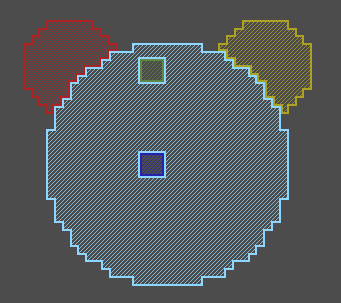
\includegraphics[width=0.4\textwidth]{BrainStimulation_figures/mickey_mouse_seg.png}
\caption{ Toy example - Mickey mouse segmentation (depicted tissue labels: red/light brown=left/right ear, light blue=body, dark blue/green=deep/superficial ROI) }
\label{fig:sim_setting}
\end{figure}

\newpage

\subsection{Generating finite element meshed (FEM) within SCIRun5 from segmentations}
The SCIRun5 network shown in \ref{fig:mesh1} implements a way to generate a tehtrahedral mesh based on a segmentation (*.nrrd file) that need to be loaded so that the data elements
are defined on the elements. The loaded field will be separated based on the label values (1..6) and for each a triangle surface is generated.
To create a valid input for the meshing tool cleaver 1.0 (module: InterfaceToCleaver) all triangle surfaces need to be represented implicitly as indicator functions.
Those indicator functions can be defined as signed distances to the surfaces of the materials. The creation of signed distance fields requires a regular grid where the signed distances are stored.
That grid (module "CreateLatVol") is created in the top part of this network and aligned with the segmentation (module "AlignMeshBoundingBoxes") as well.

\begin{figure}[!h]
\centering
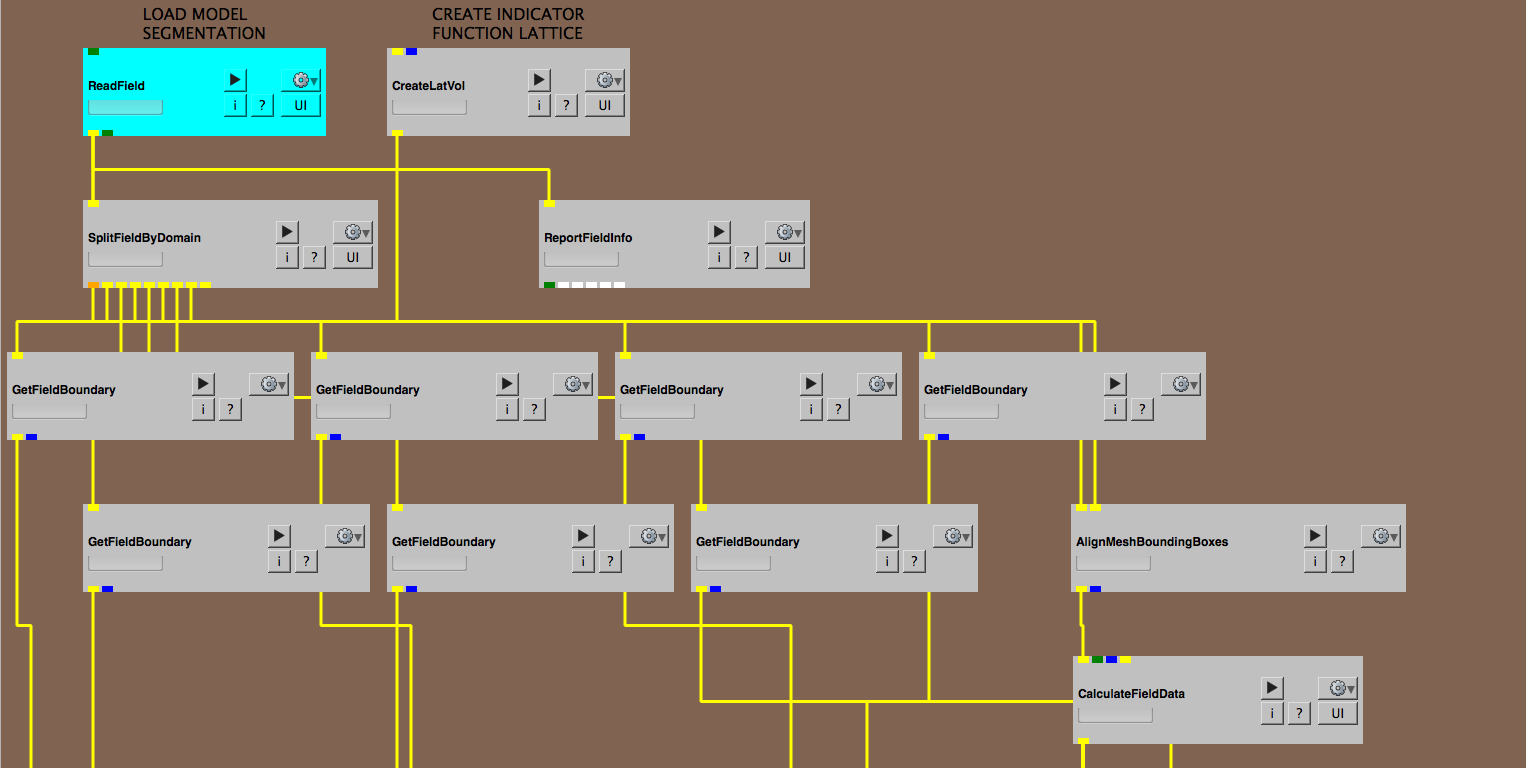
\includegraphics[width=1.0\textwidth]{BrainStimulation_figures/make_mesh1.png}
\caption{ Mickey mouse segmentation: Tetrahedral mesh generation, SCIRun5 network (1/2) }
\label{fig:mesh1}
\end{figure}

The second part of the network (\ref{fig:mesh2}) takes all tissue surfaces and the regular grid (latvol) to compute signed distances that will serve as indicator functions.
Each output (signed distance field) piped into a CalculateFieldData module to be converted to float. All signed distance fields are piped into Cleaver (Cleaver expects to have positive 
signed distance values inside and negative values outside of it, for each material (also background) a positive distance value needs to be defined in one input).

\begin{figure}[!h]
\centering
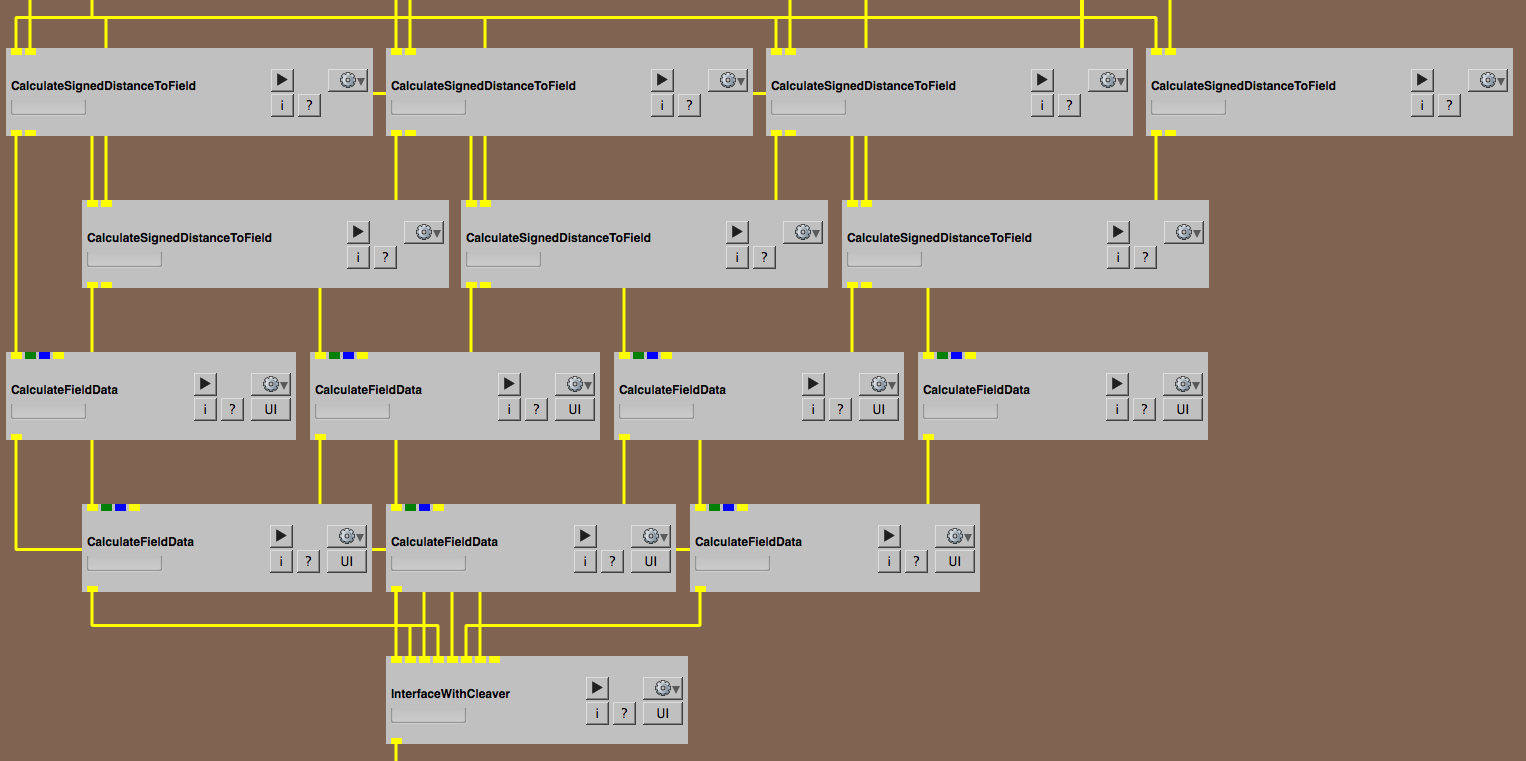
\includegraphics[width=0.8\textwidth]{BrainStimulation_figures/make_mesh2.png}
\caption{ Mickey mouse segmentation: Tetrahedral mesh generation, SCIRun5 network (2/2)}
\label{fig:mesh2}
\end{figure}


\section{Simulating Transcranial Direct Current Stimulation (tDCS)}\label{sec:sim_tdcs}
The SCIRun5 network discussed in the following can be found at \texttt{src/ExampleNets/BrainStimulator/TDCS\_TOY\_EXAMPLE.srn5}.

\subsection{SCIRun5 tDCS network: Part 1/5}
The only difference of figure \ref{fig:tdcs1} to figure \ref{fig:mesh1} are the 2 modules in the top right corner. One creates a matrix of electrode locations (x, y, z) and
the other one reads the shape of a tDCS electrode prototype.

\begin{figure}[!h]
\centering
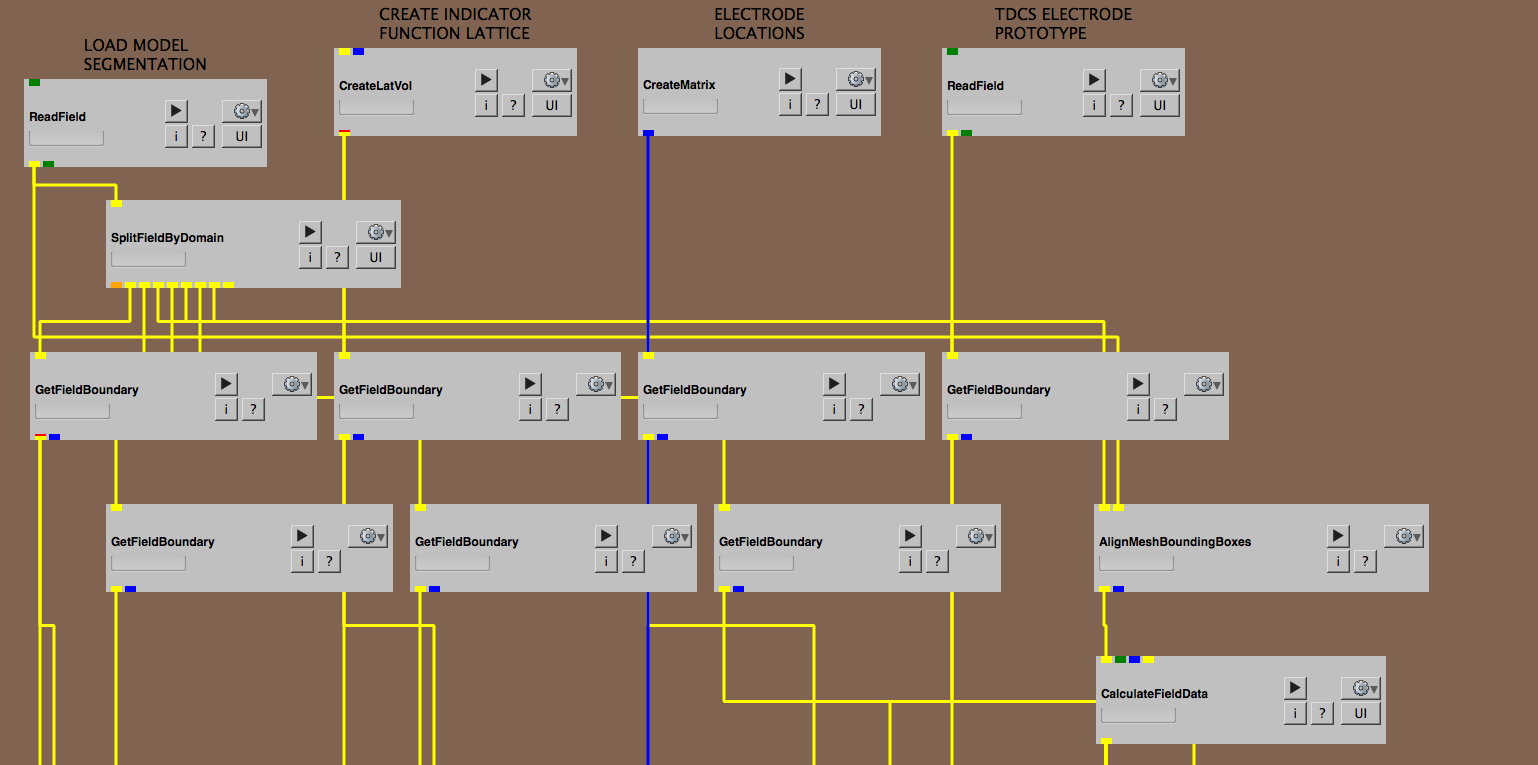
\includegraphics[width=0.8\textwidth]{BrainStimulation_figures/tdcs_1.png}
\caption{ tDCS SCIRun5 network (1/5)}
\label{fig:tdcs1}
\end{figure}

In figure \ref{fig:tdcs2}, the module ElectrodeCoilSetup is highlighted which positions each electrode on the scalp and generates a Field of definied electrode 
shapes that fit the scalp surface and can be used later to create a signed distance field for the electrodes (as an input for Cleaver). 


\begin{figure}[!h]
\centering
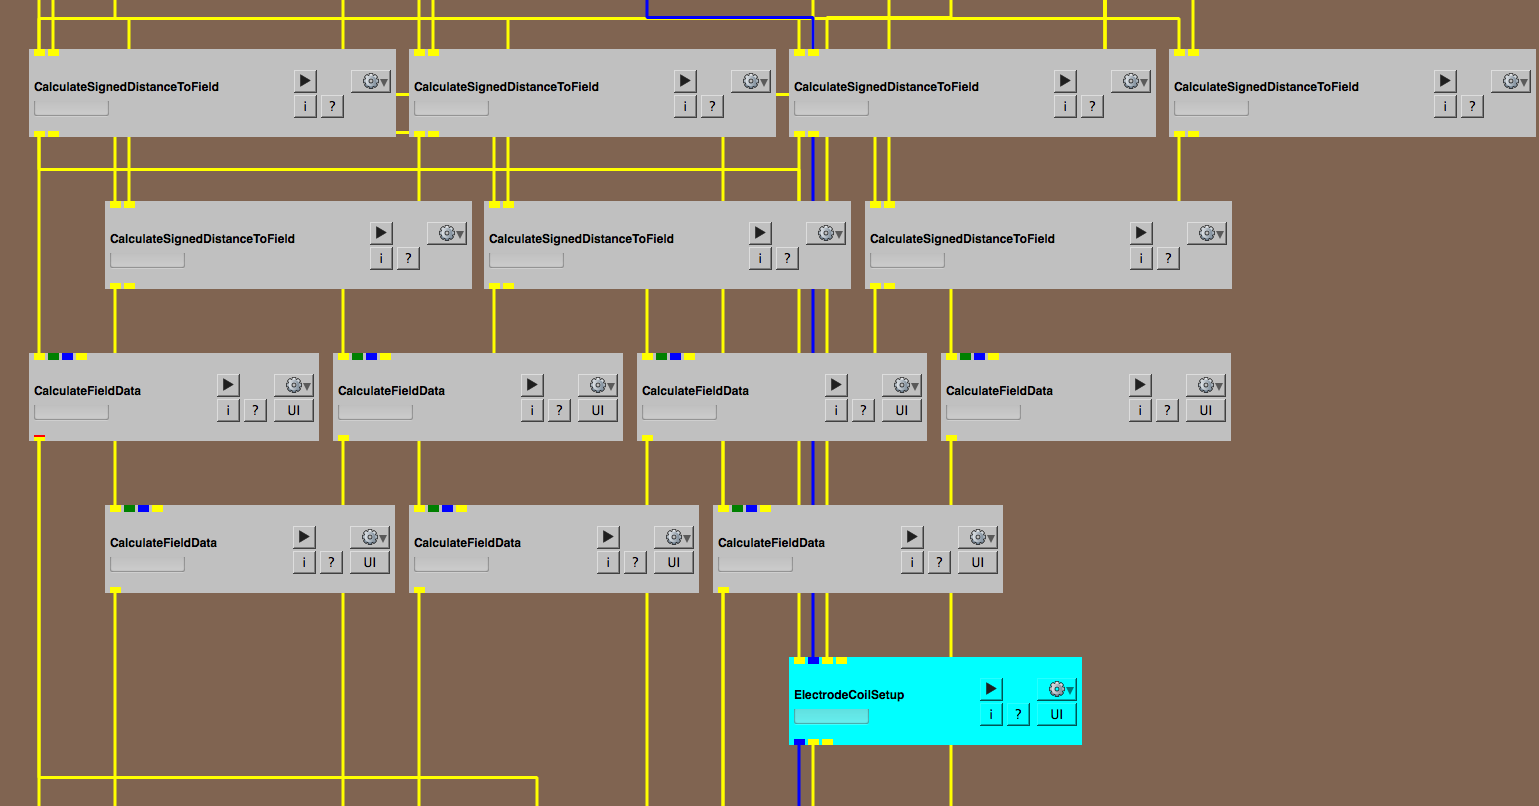
\includegraphics[width=0.8\textwidth]{BrainStimulation_figures/tdcs_2.png}
\caption{ tDCS SCIRun5 network (2/5)}
\label{fig:tdcs2}
\end{figure}

Figure \ref{fig:tdcs3} demonstrates this process of the model mesh generation is performed by the InterfaceWithCleaver module that takes all tissues as well as
the electrode inputs (signed distance fields) and outputs a tetrahedral mesh. This tetrahedral mesh is split into labels whereas the background,
which is not needed for computations, is stripped. The scalp and electrode tissue surfaces are created to set up FEM computations.

\begin{figure}[!h]
\centering
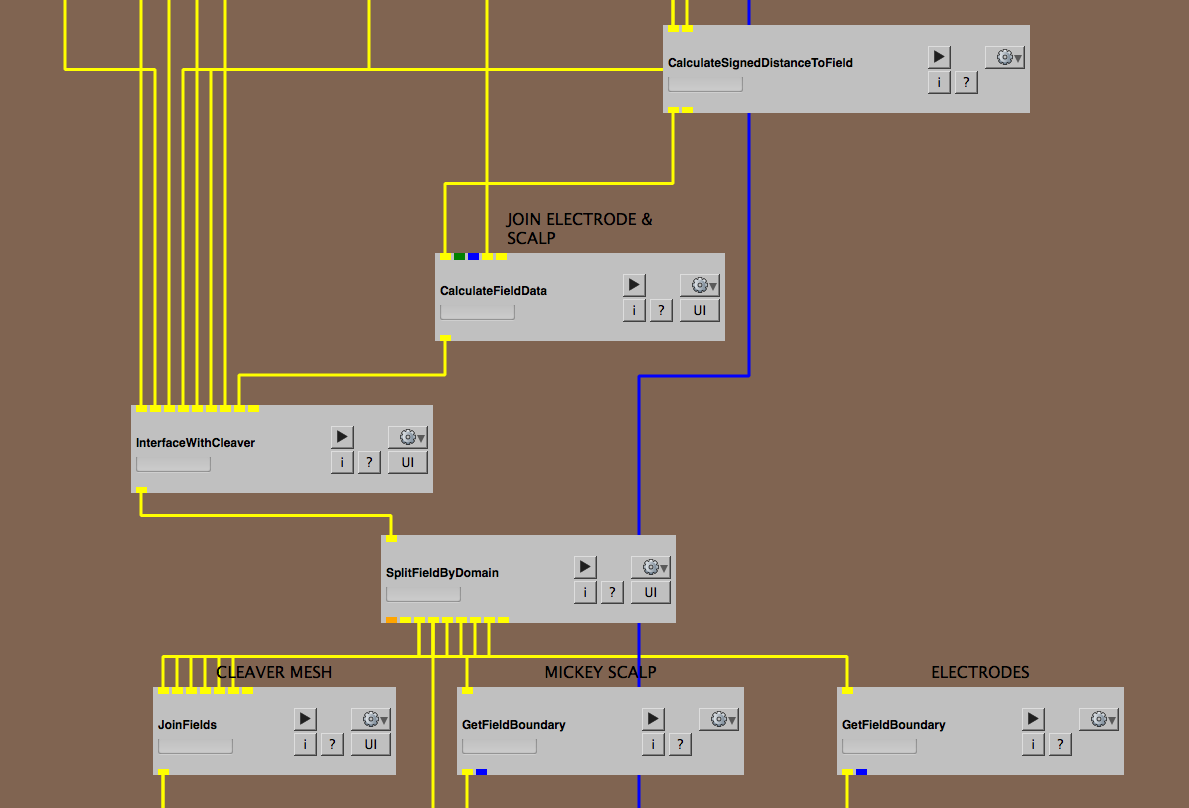
\includegraphics[width=0.8\textwidth]{BrainStimulation_figures/tdcs_3.png}
\caption{ tDCS SCIRun5 network (3/5)}
\label{fig:tdcs2}
\end{figure}

In figure \ref{fig:tdcs4} presents the computation core of the network. The created tetraherdral mesh is populated with
isotropic conductivity values from the SetMeshConductivities module (user input possible to change conductivities) and piped directly into the BuildFEMatrix module
to generate the FEM stiffness matrix $A_{1}$. The module SetupTDCS takes all the information on the tDCS electrode definition and creates
outputs to be able to set appropriate electrical boundary conditions (user input possible to define electrode current intensities and reference node).
Those outputs are piped mainly into the module BuildTDCSMatrix to create the TDCS forward matrix $A$. $A$ and $I$ (SetupTDCS) are piped into SolveLinearSystem
to solve $A\ \cdot\ U\ =\ I$ iteratively for the potential vector $U$.

\begin{figure}[!h]
\centering
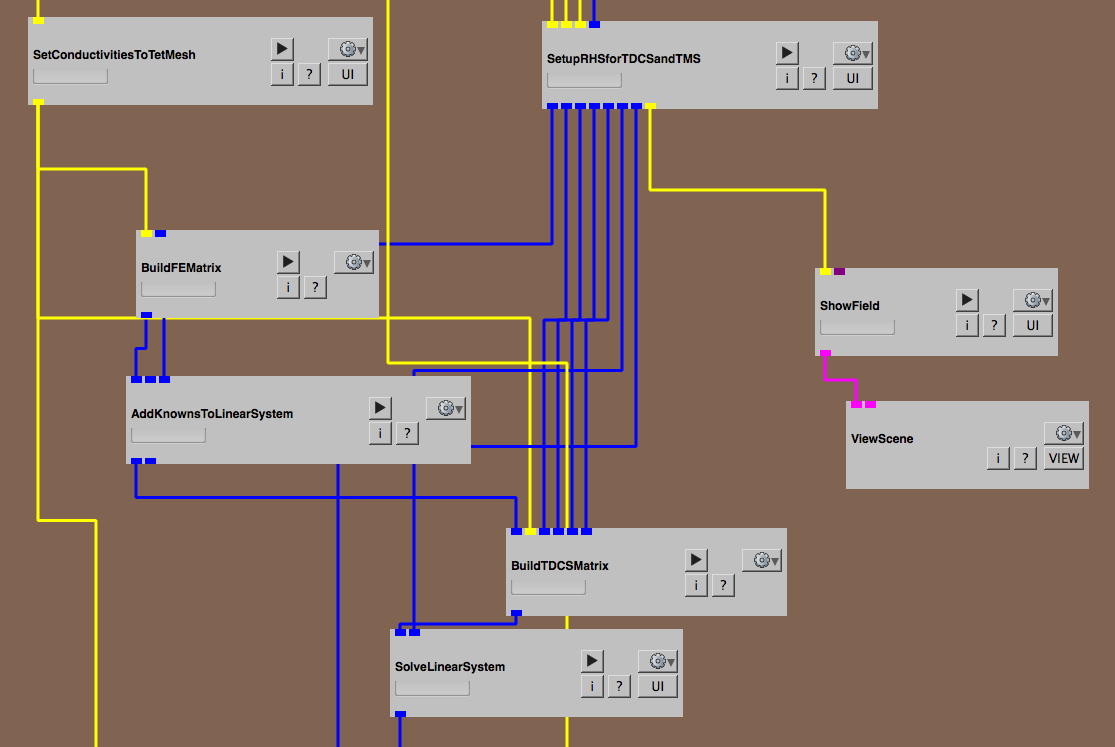
\includegraphics[width=0.8\textwidth]{BrainStimulation_figures/tdcs_4.png}
\caption{ tDCS SCIRun5 network (4/5)}
\label{fig:tdcs2}
\end{figure}


The computed solution $U$ is split into the nodal potential vector $U_n$ that is only needed for further computations (figure \ref{fig:tdcs5}).
Then, the nodal potentials are assined to the previously generated tetrahedral mesh and mapped onto a triangle surface (here Mickey's body) for inspection.
The mapped potentials defined on Mickey's body surface are mapped to its nodes in order to be visualized in ViewScene.

 \begin{figure}[!h]
\centering
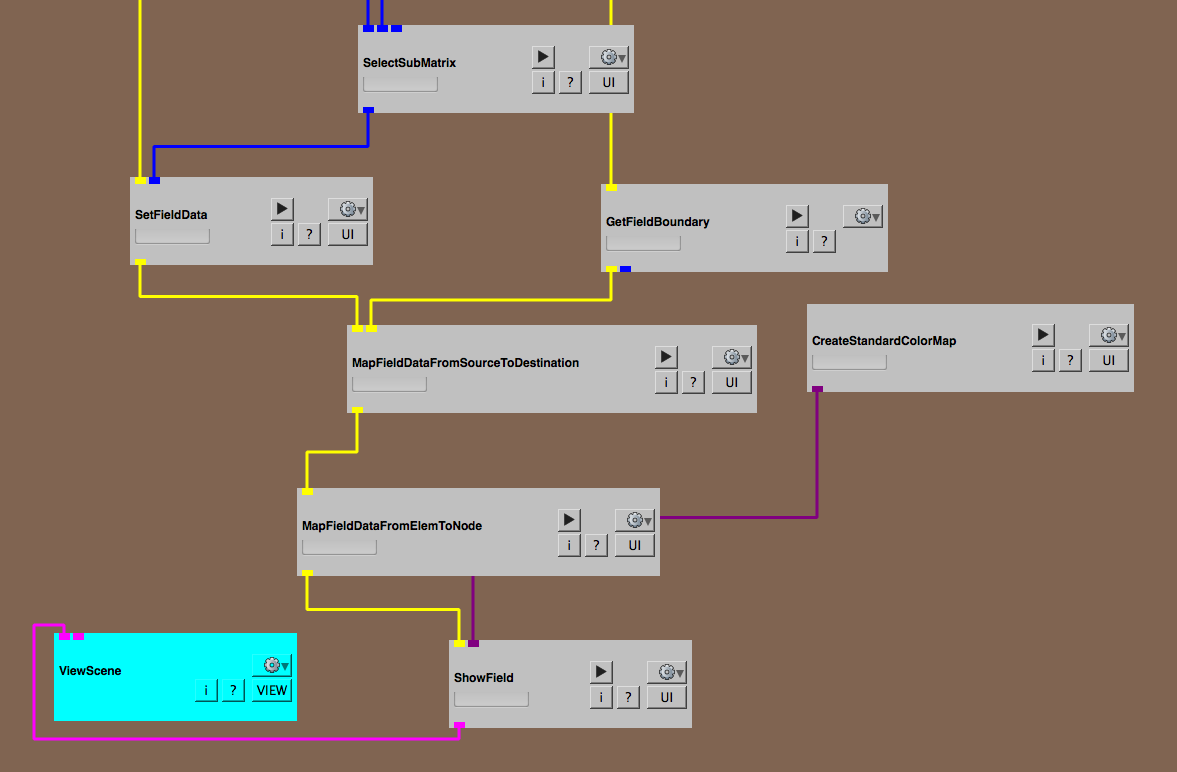
\includegraphics[width=0.8\textwidth]{BrainStimulation_figures/tdcs_5.png}
\caption{ tDCS SCIRun5 network (5/5)}
\label{fig:tdcs5}
\end{figure}

\section{Simulating Transcranial Magnetic Stimulation (TMS)}\label{sec:sim_tms}
The SCIRun5 network discussed in the following can be found at \texttt{src/ExampleNets/BrainStimulator/TMS\_TOY\_EXAMPLE.srn5}.
As previously described, the tetrahedral mesh is created in a similar fashion from the segmentation.
In figure \ref{fig:tms1}, the TMS coil location is defined and the tms coil prototype is loaded. The magnetically induced primary current
is computed and a finite element mesh is set up. The primary current is fed into the BuildFEVolRHS to set up the volumetric primary currents (right hand side)
to solve for the secondary currents.

 \begin{figure}[!h]
\centering
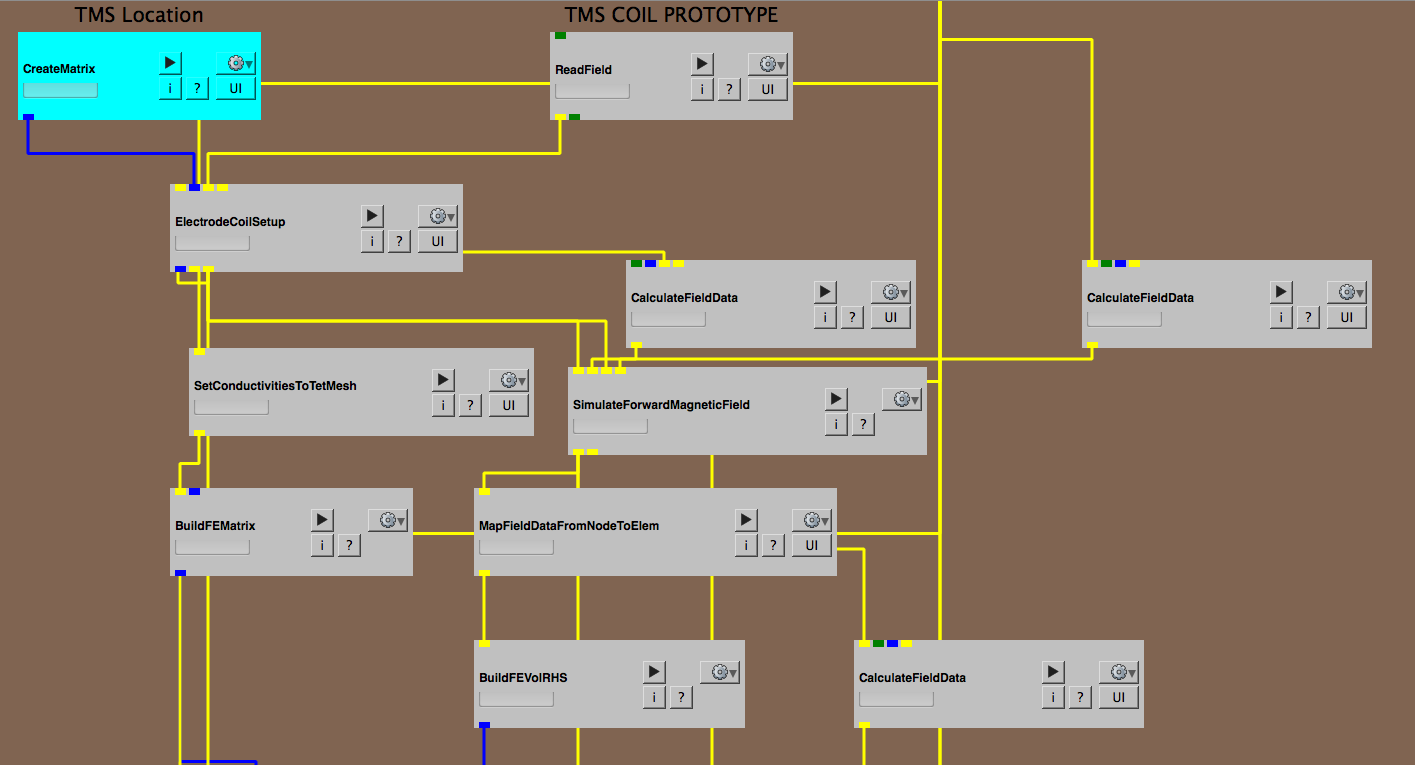
\includegraphics[width=0.8\textwidth]{BrainStimulation_figures/tms1.png}
\caption{ TMS SCIRun5 network (1/4)}
\label{fig:tms1}
\end{figure}

In figure \ref{fig:tms2}, the secondary currents are solved and electrical gradients are calculated.

 \begin{figure}[!h]
\centering
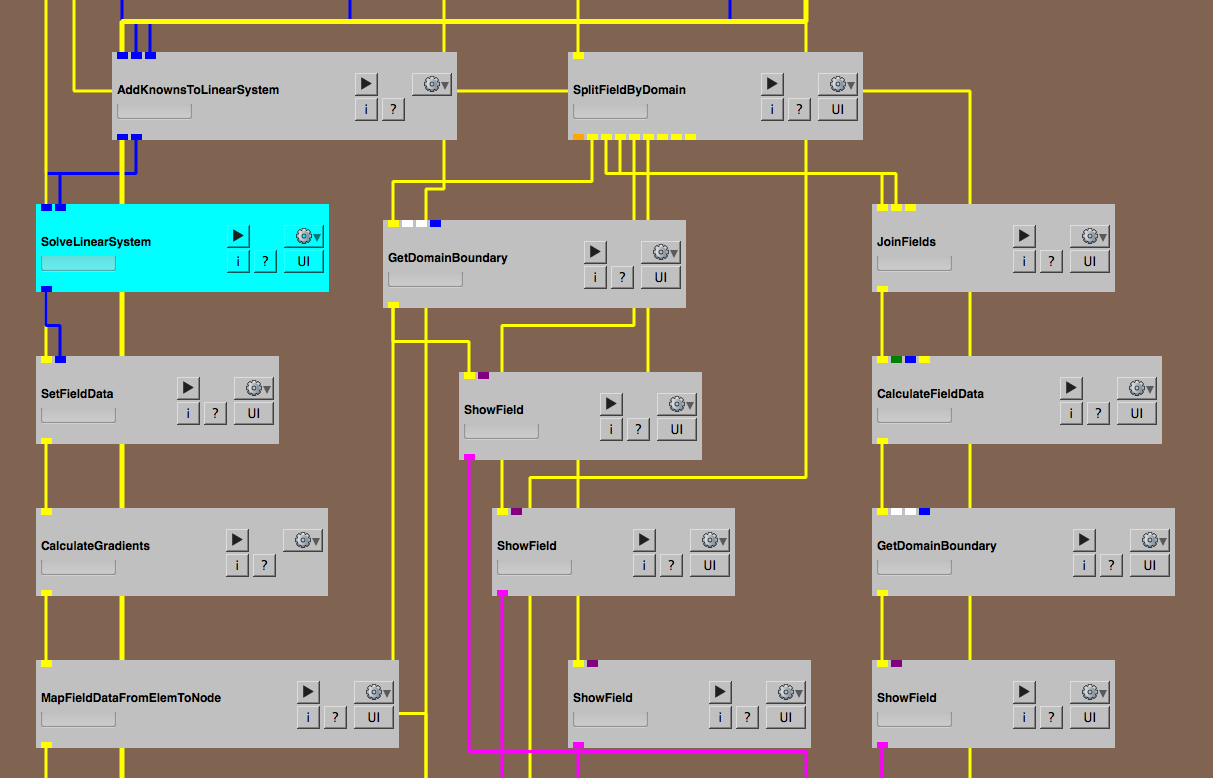
\includegraphics[width=0.8\textwidth]{BrainStimulation_figures/tms2.png}
\caption{ RMS SCIRun5 network (2/4)}
\label{fig:tms2}
\end{figure}

In figure \ref{fig:tms3}, primary and secondary currents are joined and mapped to the mesh.

 \begin{figure}[!h]
\centering
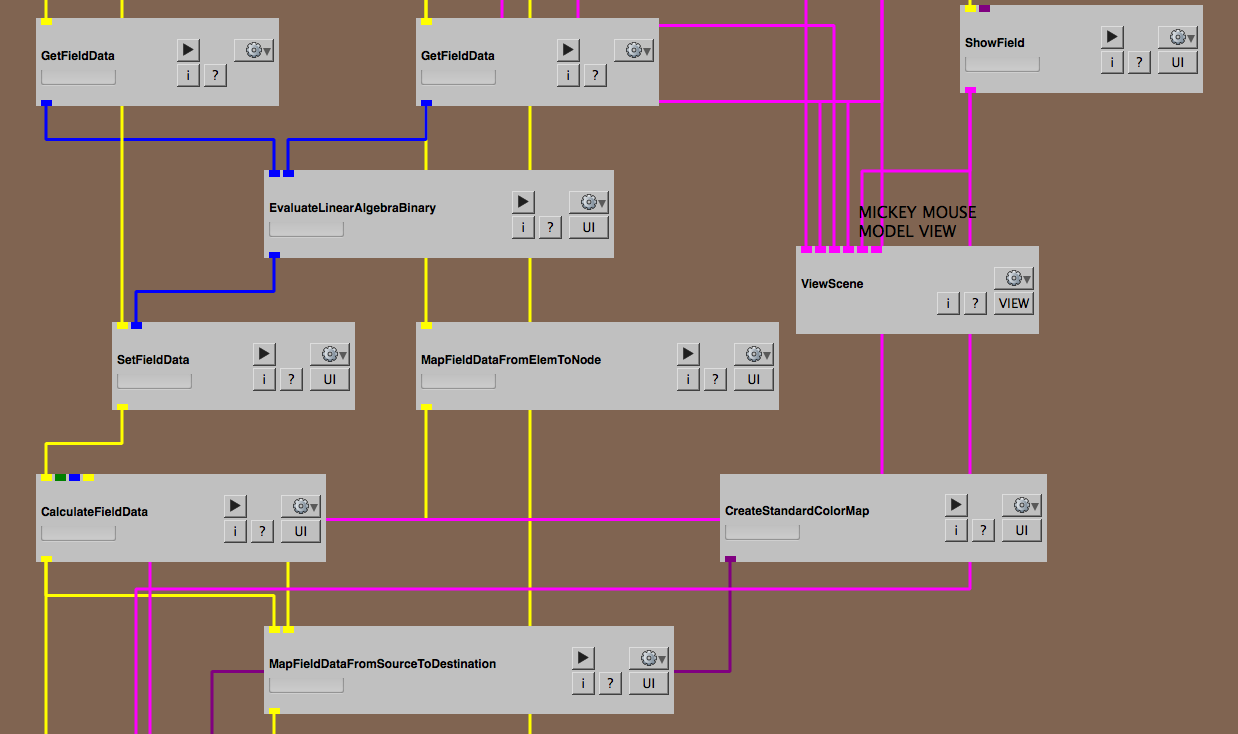
\includegraphics[width=0.8\textwidth]{BrainStimulation_figures/tms3.png}
\caption{ RMS SCIRun5 network (3/4)}
\label{fig:tms3}
\end{figure}

In figure \ref{fig:tms4}, the currents are mapped to Mickey's body and ROI based analysis can be performed.


 \begin{figure}[!h]
\centering
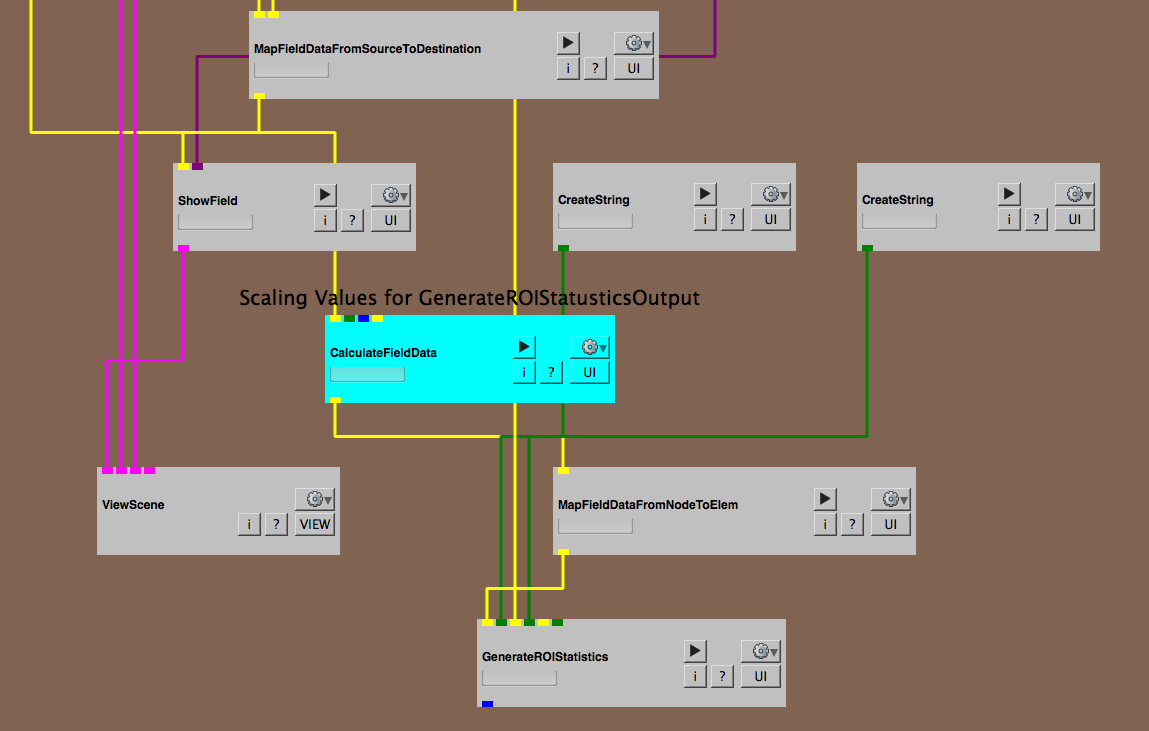
\includegraphics[width=0.8\textwidth]{BrainStimulation_figures/tms4.png}
\caption{ RMS SCIRun5 network (4/4)}
\label{fig:tms4}
\end{figure}

\chapter{Appendix}

\section{Modules}

Modules are the workhorses of SCIRun. Below is given a brief description of the modules used in this tutorial. To obtain a complete understanding for each module visit \href{http://www.sci.utah.edu/software/scirun.html}{SCIRun documentation}.

\subsection{ElectrodeCoilSetup}
\begin{figure}[!h]
	\centering
	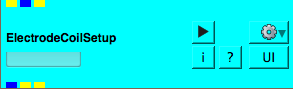
\includegraphics[width=\imgSm\textwidth]{BrainStimulation_figures/ElectrodeCoilSetup.png}
	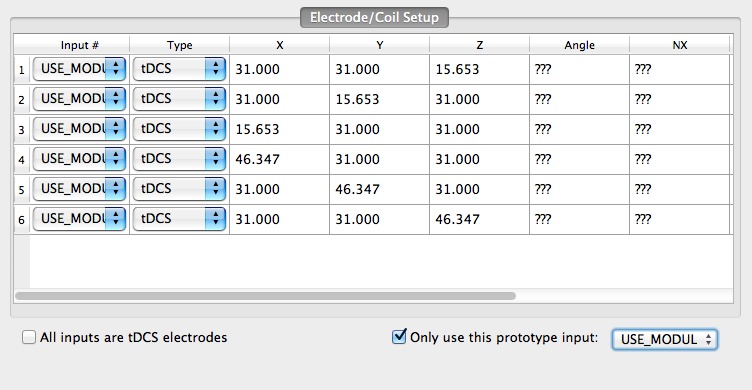
\includegraphics[width=0.95\textwidth]{BrainStimulation_figures/ElectrodeCoilSetup_GUI.png}
	\caption{Electrode / coil setup module allows for electrode or magnetic coils properties to be manually inputed, such as the height, width, and length.}
	\label{fig:elec_coil_setup}
\end{figure}

 

\subsection{SetupTDCS}
\begin{figure}[!h]
	\centering
	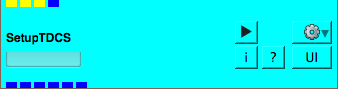
\includegraphics[width=\imgSm\textwidth]{BrainStimulation_figures/SetupTDCS.png}
	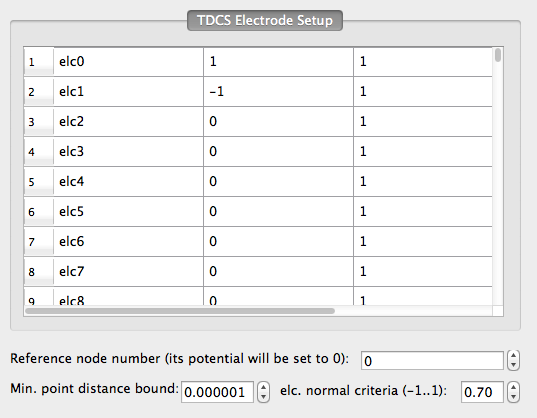
\includegraphics[width=0.8\textwidth]{BrainStimulation_figures/SetupTDCS_GUI.png}
	\caption{SetupRHSforTDCSandTMS module allows the desired current intensity and impedance for individual electrodes to be set manually. The reference electrode is also able to be specified by the row number in the table.}
	\label{fig:setup_rhs}
\end{figure}

\subsection{GenerateROIStatistics}
\begin{figure}[!h]
	\centering
	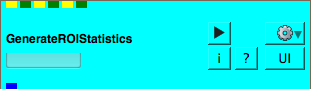
\includegraphics[width=\imgSm\textwidth]{BrainStimulation_figures/generateroistatistics.png}
	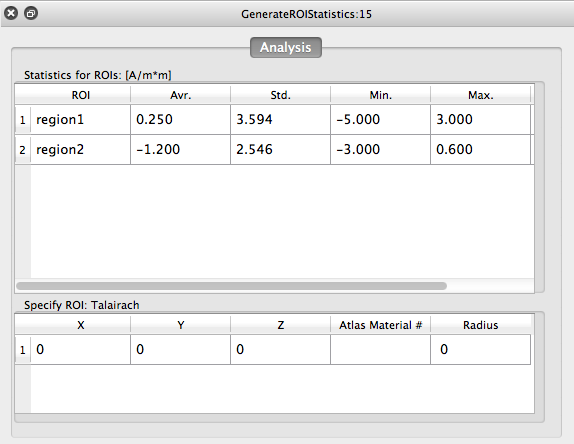
\includegraphics[width=0.8\textwidth]{BrainStimulation_figures/generateroistatistics_GUI.png}
	\caption{GenerateROIStatistics module calculates the average, standard deviation, maximum, and minimum of the current density at desired ROIs. ROIs are specified by x, y, z marker and a radius which is used to create a sphere from the point specified.}
	\label{fig:gen_roi_statistics}
\end{figure}

\subsection{SetMeshConductivities}
\begin{figure}[!h]
	\centering
	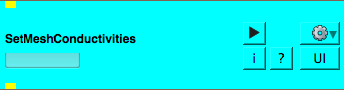
\includegraphics[width=\imgSm\textwidth]{BrainStimulation_figures/SetMeshConductivities.png}
	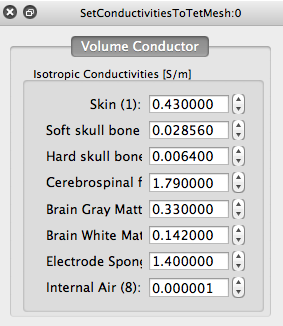
\includegraphics[width=\imgSm\textwidth]{BrainStimulation_figures/SetMeshConductivities_GUI.png}
	\caption{This module allows you to set conductivity values for different fields contained within the mesh. The fields that are available for changing are: skin, soft skull bone, hard skull bone, cerebral spinal fluid, brain gray matter, brain white matter, electrode sponge, and internal air.}
	\label{fig:set_conductivities_tet_mesh}
\end{figure}

\end{document}
